\documentclass[]{book}
\usepackage{lmodern}
\usepackage{amssymb,amsmath}
\usepackage{ifxetex,ifluatex}
\usepackage{fixltx2e} % provides \textsubscript
\ifnum 0\ifxetex 1\fi\ifluatex 1\fi=0 % if pdftex
  \usepackage[T1]{fontenc}
  \usepackage[utf8]{inputenc}
\else % if luatex or xelatex
  \ifxetex
    \usepackage{mathspec}
  \else
    \usepackage{fontspec}
  \fi
  \defaultfontfeatures{Ligatures=TeX,Scale=MatchLowercase}
\fi
% use upquote if available, for straight quotes in verbatim environments
\IfFileExists{upquote.sty}{\usepackage{upquote}}{}
% use microtype if available
\IfFileExists{microtype.sty}{%
\usepackage{microtype}
\UseMicrotypeSet[protrusion]{basicmath} % disable protrusion for tt fonts
}{}
\usepackage[margin=1in]{geometry}
\usepackage{hyperref}
\hypersetup{unicode=true,
            pdftitle={FACE Benchmarking Project Documentation},
            pdfauthor={Betsy Cowdery},
            pdfborder={0 0 0},
            breaklinks=true}
\urlstyle{same}  % don't use monospace font for urls
\usepackage{natbib}
\bibliographystyle{plainnat}
\usepackage{color}
\usepackage{fancyvrb}
\newcommand{\VerbBar}{|}
\newcommand{\VERB}{\Verb[commandchars=\\\{\}]}
\DefineVerbatimEnvironment{Highlighting}{Verbatim}{commandchars=\\\{\}}
% Add ',fontsize=\small' for more characters per line
\usepackage{framed}
\definecolor{shadecolor}{RGB}{248,248,248}
\newenvironment{Shaded}{\begin{snugshade}}{\end{snugshade}}
\newcommand{\AlertTok}[1]{\textcolor[rgb]{0.94,0.16,0.16}{#1}}
\newcommand{\AnnotationTok}[1]{\textcolor[rgb]{0.56,0.35,0.01}{\textbf{\textit{#1}}}}
\newcommand{\AttributeTok}[1]{\textcolor[rgb]{0.77,0.63,0.00}{#1}}
\newcommand{\BaseNTok}[1]{\textcolor[rgb]{0.00,0.00,0.81}{#1}}
\newcommand{\BuiltInTok}[1]{#1}
\newcommand{\CharTok}[1]{\textcolor[rgb]{0.31,0.60,0.02}{#1}}
\newcommand{\CommentTok}[1]{\textcolor[rgb]{0.56,0.35,0.01}{\textit{#1}}}
\newcommand{\CommentVarTok}[1]{\textcolor[rgb]{0.56,0.35,0.01}{\textbf{\textit{#1}}}}
\newcommand{\ConstantTok}[1]{\textcolor[rgb]{0.00,0.00,0.00}{#1}}
\newcommand{\ControlFlowTok}[1]{\textcolor[rgb]{0.13,0.29,0.53}{\textbf{#1}}}
\newcommand{\DataTypeTok}[1]{\textcolor[rgb]{0.13,0.29,0.53}{#1}}
\newcommand{\DecValTok}[1]{\textcolor[rgb]{0.00,0.00,0.81}{#1}}
\newcommand{\DocumentationTok}[1]{\textcolor[rgb]{0.56,0.35,0.01}{\textbf{\textit{#1}}}}
\newcommand{\ErrorTok}[1]{\textcolor[rgb]{0.64,0.00,0.00}{\textbf{#1}}}
\newcommand{\ExtensionTok}[1]{#1}
\newcommand{\FloatTok}[1]{\textcolor[rgb]{0.00,0.00,0.81}{#1}}
\newcommand{\FunctionTok}[1]{\textcolor[rgb]{0.00,0.00,0.00}{#1}}
\newcommand{\ImportTok}[1]{#1}
\newcommand{\InformationTok}[1]{\textcolor[rgb]{0.56,0.35,0.01}{\textbf{\textit{#1}}}}
\newcommand{\KeywordTok}[1]{\textcolor[rgb]{0.13,0.29,0.53}{\textbf{#1}}}
\newcommand{\NormalTok}[1]{#1}
\newcommand{\OperatorTok}[1]{\textcolor[rgb]{0.81,0.36,0.00}{\textbf{#1}}}
\newcommand{\OtherTok}[1]{\textcolor[rgb]{0.56,0.35,0.01}{#1}}
\newcommand{\PreprocessorTok}[1]{\textcolor[rgb]{0.56,0.35,0.01}{\textit{#1}}}
\newcommand{\RegionMarkerTok}[1]{#1}
\newcommand{\SpecialCharTok}[1]{\textcolor[rgb]{0.00,0.00,0.00}{#1}}
\newcommand{\SpecialStringTok}[1]{\textcolor[rgb]{0.31,0.60,0.02}{#1}}
\newcommand{\StringTok}[1]{\textcolor[rgb]{0.31,0.60,0.02}{#1}}
\newcommand{\VariableTok}[1]{\textcolor[rgb]{0.00,0.00,0.00}{#1}}
\newcommand{\VerbatimStringTok}[1]{\textcolor[rgb]{0.31,0.60,0.02}{#1}}
\newcommand{\WarningTok}[1]{\textcolor[rgb]{0.56,0.35,0.01}{\textbf{\textit{#1}}}}
\usepackage{longtable,booktabs}
\usepackage{graphicx,grffile}
\makeatletter
\def\maxwidth{\ifdim\Gin@nat@width>\linewidth\linewidth\else\Gin@nat@width\fi}
\def\maxheight{\ifdim\Gin@nat@height>\textheight\textheight\else\Gin@nat@height\fi}
\makeatother
% Scale images if necessary, so that they will not overflow the page
% margins by default, and it is still possible to overwrite the defaults
% using explicit options in \includegraphics[width, height, ...]{}
\setkeys{Gin}{width=\maxwidth,height=\maxheight,keepaspectratio}
\IfFileExists{parskip.sty}{%
\usepackage{parskip}
}{% else
\setlength{\parindent}{0pt}
\setlength{\parskip}{6pt plus 2pt minus 1pt}
}
\setlength{\emergencystretch}{3em}  % prevent overfull lines
\providecommand{\tightlist}{%
  \setlength{\itemsep}{0pt}\setlength{\parskip}{0pt}}
\setcounter{secnumdepth}{5}
% Redefines (sub)paragraphs to behave more like sections
\ifx\paragraph\undefined\else
\let\oldparagraph\paragraph
\renewcommand{\paragraph}[1]{\oldparagraph{#1}\mbox{}}
\fi
\ifx\subparagraph\undefined\else
\let\oldsubparagraph\subparagraph
\renewcommand{\subparagraph}[1]{\oldsubparagraph{#1}\mbox{}}
\fi

%%% Use protect on footnotes to avoid problems with footnotes in titles
\let\rmarkdownfootnote\footnote%
\def\footnote{\protect\rmarkdownfootnote}

%%% Change title format to be more compact
\usepackage{titling}

% Create subtitle command for use in maketitle
\providecommand{\subtitle}[1]{
  \posttitle{
    \begin{center}\large#1\end{center}
    }
}

\setlength{\droptitle}{-2em}

  \title{FACE Benchmarking Project Documentation}
    \pretitle{\vspace{\droptitle}\centering\huge}
  \posttitle{\par}
    \author{Betsy Cowdery}
    \preauthor{\centering\large\emph}
  \postauthor{\par}
      \predate{\centering\large\emph}
  \postdate{\par}
    \date{2019-10-28}

\usepackage{booktabs}

\begin{document}
\maketitle

{
\setcounter{tocdepth}{1}
\tableofcontents
}
\hypertarget{documentation}{%
\chapter{Documentation}\label{documentation}}

This is all the documentation that will also hopefullt become the paper.

\hypertarget{setup}{%
\chapter*{Setup}\label{setup}}
\addcontentsline{toc}{chapter}{Setup}

\begin{Shaded}
\begin{Highlighting}[]
\CommentTok{##########################}
\CommentTok{# Get all the ids for BETY }

\CommentTok{# load in the current json file}
\NormalTok{ids <-}\StringTok{ }\NormalTok{rjson}\OperatorTok{::}\KeywordTok{fromJSON}\NormalTok{(}\DataTypeTok{file =} \StringTok{"/fs/data3/ecowdery/FACE/FACE-MDS_runs/ids.json"}\NormalTok{)}

\CommentTok{# run ids}
\NormalTok{runs <-}\StringTok{ }\NormalTok{dplyr}\OperatorTok{::}\KeywordTok{bind_rows}\NormalTok{(ids}\OperatorTok{$}\NormalTok{runs, }\DataTypeTok{.id =} \StringTok{"model"}\NormalTok{) }\OperatorTok\StringTok{ }
\StringTok{  }\KeywordTok{gather}\NormalTok{(}\DataTypeTok{key=}\StringTok{"treatment"}\NormalTok{, }\DataTypeTok{value =}\StringTok{"workflow_id"}\NormalTok{, }\OperatorTok{-}\StringTok{"model"}\NormalTok{)}

\CommentTok{# I selected these variables because they are the most common / interesting}
\CommentTok{# But there may be more that we want to include in the future ...}
\NormalTok{vars <-}\StringTok{ }\KeywordTok{c}\NormalTok{(}\StringTok{"NEE"}\NormalTok{, }\StringTok{"TotalResp"}\NormalTok{, }\StringTok{"Qle"}\NormalTok{, }\StringTok{"NPP"}\NormalTok{, }\StringTok{"LAI"}\NormalTok{, }\StringTok{"SoilMoistFrac"}\NormalTok{, }\StringTok{"TotLivBiom"}\NormalTok{)}

\CommentTok{# input ids}
\NormalTok{inputs <-}\StringTok{ }\NormalTok{dplyr}\OperatorTok{::}\KeywordTok{bind_rows}\NormalTok{(ids}\OperatorTok{$}\NormalTok{inputs) }\OperatorTok\StringTok{ }
\StringTok{  }\KeywordTok{gather}\NormalTok{(}\DataTypeTok{key =} \StringTok{"input_name"}\NormalTok{, }\DataTypeTok{value =} \StringTok{"input_id"}\NormalTok{)}

\NormalTok{bety <-}\StringTok{ }\KeywordTok{betyConnect}\NormalTok{(}\StringTok{"/fs/data3/ecowdery/pecan/web/config.php"}\NormalTok{)}
\NormalTok{inputs <-}\StringTok{ }\NormalTok{inputs }\OperatorTok\StringTok{ }
\StringTok{  }\KeywordTok{left_join}\NormalTok{(}\KeywordTok{tbl}\NormalTok{(bety, }\StringTok{"inputs"}\NormalTok{) }\OperatorTok\StringTok{ }\KeywordTok{filter}\NormalTok{(id }\OperatorTok\StringTok{ }\NormalTok{inputs}\OperatorTok{$}\NormalTok{input_id) }\OperatorTok\StringTok{ }\KeywordTok{select}\NormalTok{(id, format_id) }\OperatorTok\StringTok{ }\KeywordTok{collect}\NormalTok{(), }
            \DataTypeTok{by =} \KeywordTok{c}\NormalTok{(}\StringTok{"input_id"}\NormalTok{ =}\StringTok{ "id"}\NormalTok{)) }\OperatorTok\StringTok{ }
\StringTok{  }\KeywordTok{left_join}\NormalTok{(}\KeywordTok{tbl}\NormalTok{(bety,}\StringTok{"formats_variables"}\NormalTok{) }\OperatorTok\StringTok{ }\KeywordTok{select}\NormalTok{(variable_id, format_id) }\OperatorTok\StringTok{ }\KeywordTok{collect}\NormalTok{()) }\OperatorTok\StringTok{ }
\StringTok{  }\KeywordTok{left_join}\NormalTok{(}\KeywordTok{tbl}\NormalTok{(bety, }\StringTok{"variables"}\NormalTok{) }\OperatorTok\StringTok{ }\KeywordTok{select}\NormalTok{(id, name) }\OperatorTok\StringTok{ }\KeywordTok{collect}\NormalTok{(), }\DataTypeTok{by =} \KeywordTok{c}\NormalTok{(}\StringTok{"variable_id"}\NormalTok{ =}\StringTok{ "id"}\NormalTok{))}
\end{Highlighting}
\end{Shaded}

\begin{verbatim}
## Joining, by = "format_id"
\end{verbatim}

\hypertarget{timeseries-plots}{%
\chapter*{Timeseries Plots}\label{timeseries-plots}}
\addcontentsline{toc}{chapter}{Timeseries Plots}

\hypertarget{npp}{%
\section*{NPP}\label{npp}}
\addcontentsline{toc}{section}{NPP}

\begin{verbatim}
## `geom_smooth()` using method = 'loess' and formula 'y ~ x'
\end{verbatim}

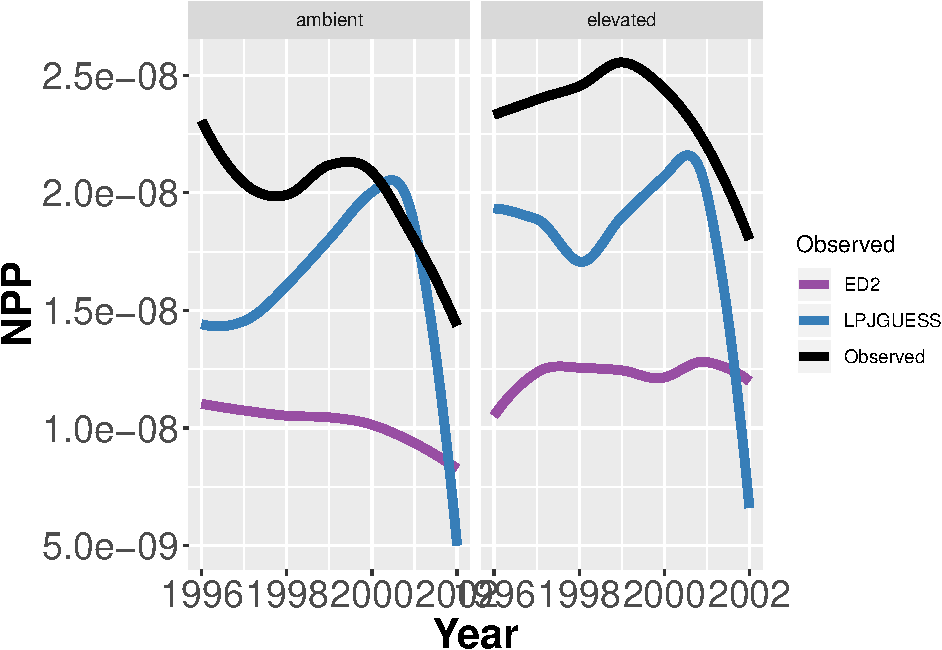
\includegraphics{FACE.docs.book_files/figure-latex/unnamed-chunk-3-1.pdf}

\hypertarget{lai}{%
\section*{LAI}\label{lai}}
\addcontentsline{toc}{section}{LAI}

\begin{verbatim}
## # A tibble: 4 x 5
##   input_name   input_id  format_id variable_id name 
##   <chr>           <dbl>      <dbl>       <dbl> <chr>
## 1 NPP_a      1000008119 1000000013          18 LAI  
## 2 NPP_e      1000008120 1000000013          18 LAI  
## 3 P2_a       1000013743 1000000061          18 LAI  
## 4 P2_e       1000013748 1000000061          18 LAI
\end{verbatim}

\begin{verbatim}
## `geom_smooth()` using method = 'loess' and formula 'y ~ x'
\end{verbatim}

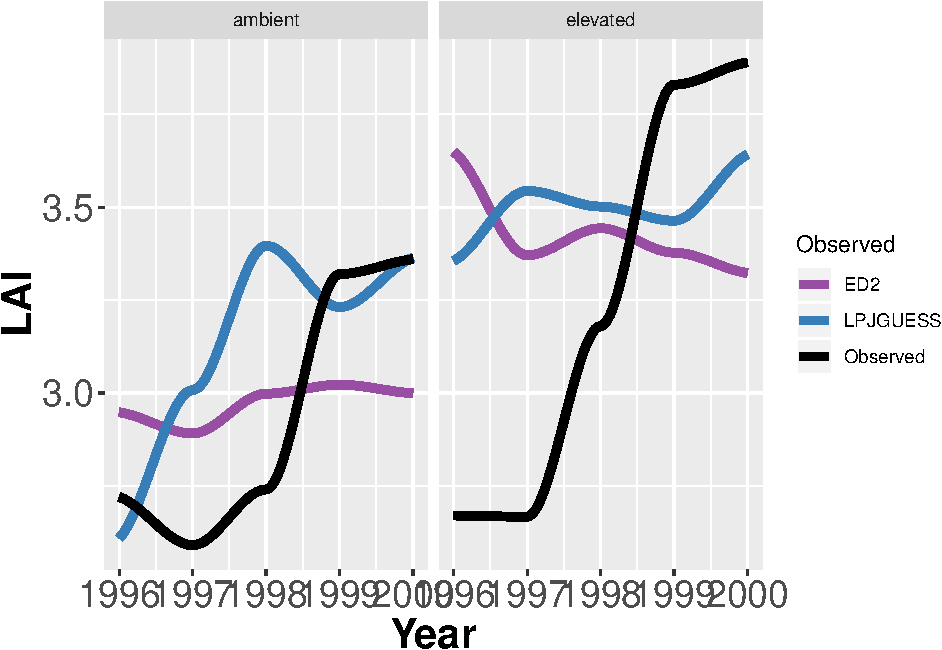
\includegraphics{FACE.docs.book_files/figure-latex/unnamed-chunk-4-1.pdf}


\end{document}
